
\section{Fundamentação Teórica}

O desenvolvimento de Veículos Aéreos Não Tripulados (VANTs) abriu caminho para arquiteturas de controle cada vez mais complexas, capazes de sustentar operações cooperativas entre múltiplos agentes. A consolidação de tecnologias como sensores inerciais, sistemas de navegação, comunicação sem fio e computação embarcada permitiu que esses veículos realizassem tarefas de forma mais autônoma e coordenada \citep{khan2017fanet}. Nesse contexto, os enxames de VANTs surgem não apenas como uma evolução da operação individual, mas como uma abordagem fundamentada em princípios de sistemas distribuídos e inteligência coletiva.

\subsection{Conceitos Básicos}

\subsubsection{VANTs e Níveis de Autonomia}

Os VANTs modernos são capazes de operar desde missões simples, guiadas remotamente, até tarefas complexas totalmente automatizadas. O que distingue esses níveis de operacionalidade é o grau de autonomia implementado em seus sistemas embarcados. Segundo a taxonomia proposta em \citep{sholes2007evolution}, os níveis de Autonomy Control Level (ACL) descrevem essa progressão, baseando-se no ciclo OODA: Observar, Orientar, Decidir e Agir — processo que define como um agente percebe o ambiente, interpreta informações e executa ações.

No nível mais baixo de autonomia, o veículo depende integralmente do operador humano, caracterizando teleoperação. Nos níveis mais elevados, funções antes atribuídas ao piloto — como planejamento de trajetórias, avaliação de contingências e tomada de decisão — são executadas de forma independente pelo sistema \citep{dong2004behavior}. Essa evolução é fundamental para operações multiagente, pois a coordenação entre vários veículos exige que cada um deles interprete o ambiente e responda sem depender de controle humano contínuo.

\subsubsection{Sistemas Multiagente e Cooperação}

A coordenação entre múltiplos VANTs é geralmente tratada no contexto de Sistemas Multiagente (MAS – Multi-Agent Systems), nos quais diversos agentes autônomos interagem para atingir um objetivo comum \citep{bu2024advancement, chung2018survey}.

A cooperação é um princípio fundamental nesses sistemas. Quando bem coordenados, múltiplos veículos simples e de baixo custo podem alcançar desempenho global superior ao de um sistema monolítico \citep{ren2007consensus}. Em um MAS aplicado a VANTs, essa cooperação exige que funções como planejamento, adaptação a falhas e reação a emergências sejam parcialmente distribuídas entre os veículos \citep{dong2004behavior}.

\subsubsection{Inteligência de Enxame}

A Inteligência de Enxame (Swarm Intelligence) é inspirada em comportamentos coletivos observados na natureza, como em colônias de formigas, bandos de pássaros ou cardumes de peixes \citep{bu2024advancement, chung2018survey}.

O princípio central da inteligência de enxame está no comportamento emergente, que resulta das interações locais entre agentes simples, sem supervisão centralizada \citep{chung2018survey}. Essa abordagem distribuída é caracterizada pela troca local de informações entre vizinhos próximos (\textit{neighbor-to-neighbor information exchange}), permitindo que cada agente atualize seu estado com base nas informações recebidas e, coletivamente, o grupo alcance um consenso global \citep{ren2007consensus, bu2024advancement}.

\subsection{Arquiteturas de Controle para Enxames de VANTs}

A arquitetura de controle define como as decisões e informações são distribuídas entre os veículos do enxame. De modo geral, essas arquiteturas podem ser classificadas em três tipos principais: centralizada, descentralizada e distribuída \citep{bu2024advancement}.

\subsubsection{Controle Centralizado}

Na arquitetura centralizada, um controlador global — geralmente uma estação terrestre ou um VANT líder — é responsável por processar todas as informações e emitir comandos para os veículos subordinados \citep{ouyang2023formation, bu2024advancement}. Uma representação dessa arquitetura é mostrada na Figura~\ref{fig:controle centralizado}.

Essa abordagem é conceitualmente simples e permite decisões consistentes, além de facilitar a otimização global. Entretanto, sofre de limitações de escalabilidade e de robustez, já que a falha do controlador central pode comprometer toda a missão \citep{bu2024advancement}. Além disso, o processamento concentrado em um único ponto gera alta carga computacional, inviabilizando o uso em enxames muito grandes \citep{ouyang2023formation}.

\begin{figure}[ht]
    \centering
    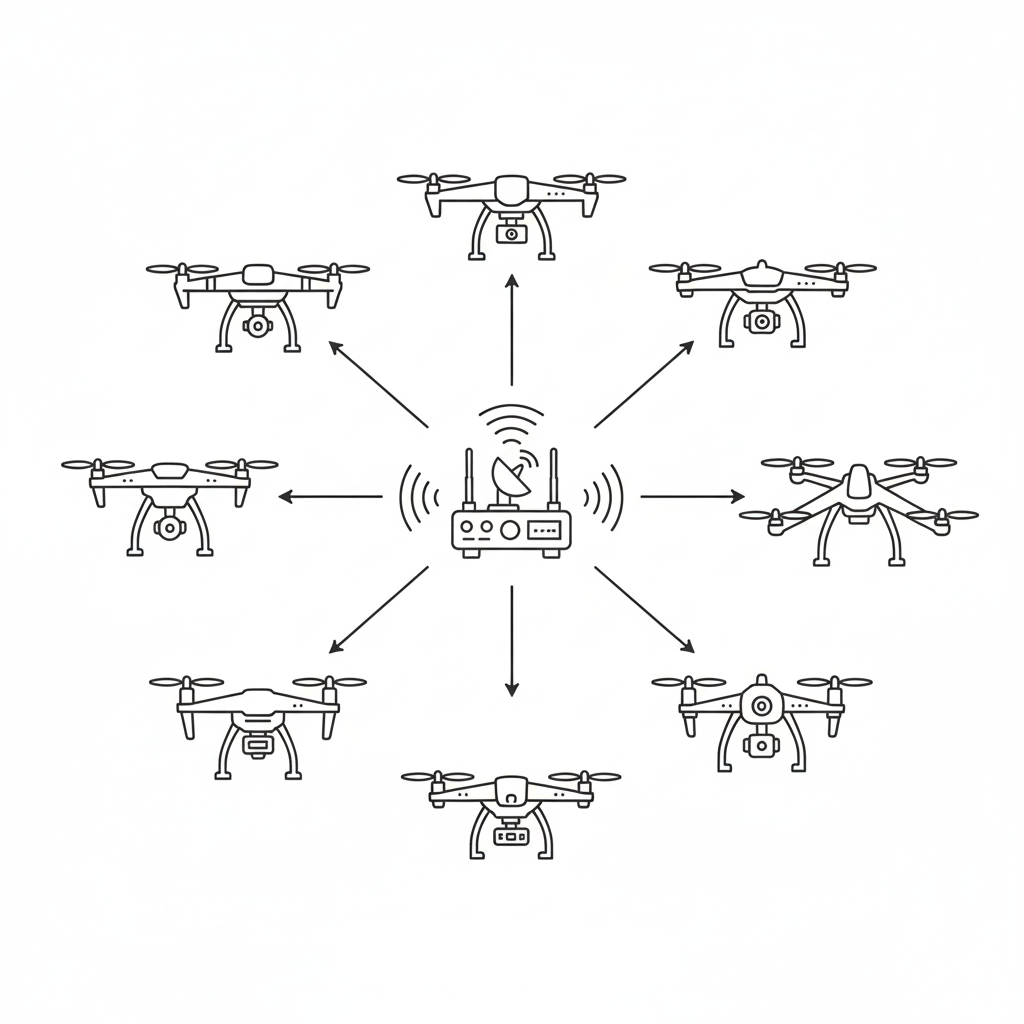
\includegraphics[width=1.0\linewidth]{images/controle centralizado.png}
    \caption{Representação do controle centralizado.}
    \label{fig:controle centralizado}
\end{figure}

\subsubsection{Controle Descentralizado e Distribuído}

No controle descentralizado, cada VANT toma decisões com base em informações locais, utilizando sensores embarcados ou comunicação com vizinhos próximos \citep{bu2024advancement}. Métodos como o \textit{Behavior-Based} e o \textit{Artificial Potential Field (APF)} são exemplos típicos dessa categoria.

Já no controle distribuído, embora não exista um centro de comando, há cooperação explícita entre os VANTs, que compartilham informações de estado para alcançar objetivos coletivos. Essa abordagem aumenta a robustez do sistema e melhora a escalabilidade, mas exige algoritmos mais complexos de consenso e sincronização \citep{bu2024advancement, ouyang2023formation}. Uma representação dessa arquitetura é mostrada na Figura~\ref{fig:controle distribuído}.

\begin{figure}[ht]
    \centering
    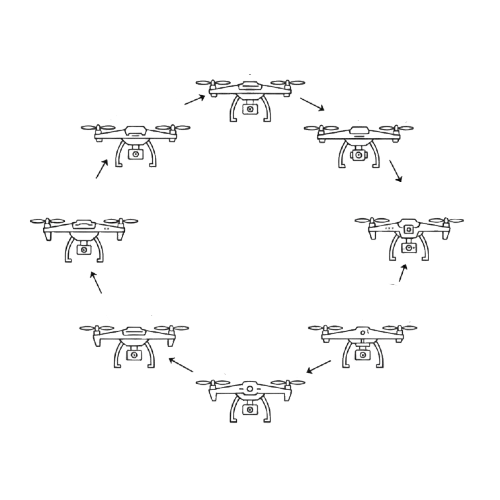
\includegraphics[width=1.0\linewidth]{images/controle distribuído rb1.png}
    \caption{Representação do controle distribuído.}
    \label{fig:controle distribuído}
\end{figure}

\subsubsection{Comparação entre Arquiteturas}

A Tabela~\ref{tab:arquiteturas-uavs} resume as principais características das arquiteturas de controle apresentadas anteriormente, destacando diferenças em robustez, escalabilidade e complexidade de implementação. Observa-se que a arquitetura centralizada apresenta baixa tolerância a falhas e escalabilidade limitada, porém sua implementação é conceitualmente mais simples. Por outro lado, arquiteturas descentralizadas ou distribuídas oferecem maior robustez e escalabilidade, mas exigem algoritmos de coordenação mais complexos, refletindo o trade-off clássico entre simplicidade de design e desempenho do sistema.


\begin{table*}[h!]
\centering
\caption{Comparação entre arquiteturas de controle em enxames de VANTs.}
\label{tab:arquiteturas-uavs}
\begin{tabular}{|p{3cm}|p{4cm}|p{3cm}|p{4cm}|}
\hline
\textbf{Estratégia} & \textbf{Robustez} & \textbf{Escalabilidade} & \textbf{Complexidade} \\ \hline
\textbf{Centralizada} & Baixa (alto risco de ponto único de falha) \citep{ouyang2023formation} & Limitada (sobrecarga computacional) \citep{bu2024advancement} & Simples (decisão unificada) \citep{bu2024advancement} \\ \hline
\textbf{Descentralizada e Distribuída} & Alta (forte tolerância a falhas) \citep{ouyang2023formation} & Alta (baseada em interações locais) \citep{bu2024advancement} & Elevada (coordenação e comunicação complexas) \citep{bu2024advancement} \\ \hline
\end{tabular}
\end{table*}


O controle distribuído tem se destacado como uma das tendências mais promissoras na pesquisa contemporânea, devido à sua robustez, flexibilidade e capacidade de escala \citep{ouyang2023formation}. Essa abordagem elimina a dependência de um ponto central e permite a coordenação emergente entre os veículos, sendo considerada a direção mais provável para o futuro das missões cooperativas com enxames de VANTs.

\subsection{Algoritmos de Formação de VANTs}

O controle de formação de VANTs consiste em coordenar o movimento de múltiplos veículos de modo que mantenham uma disposição espacial específica, geralmente representada por padrões geométricos como linha, V, triângulo ou diamante \citep{bu2024advancement}. Essa tarefa é central em aplicações cooperativas, como vigilância, mapeamento, busca e salvamento e monitoramento ambiental \citep{bu2024advancement, ouyang2023formation}.

Do ponto de vista matemático, a formação pode ser modelada considerando um conjunto de $N$ drones cuja posição linear é denotada por $p_i \in \mathbb{R}^n$. Aqui, $\mathbb{R}^n$ representa o espaço euclidiano de dimensão $n$, tipicamente $n = 2$ (espaço planar) ou $n = 3$ (espaço tridimensional).

As grandezas introduzidas nesta seção — $p_i$, $p_j$, $v_i$, $v_j$ — referem-se exclusivamente às componentes lineares da dinâmica dos VANTs. Variáveis angulares, tais como orientação e taxas de rotação, não são consideradas neste modelo específico, o qual foca apenas no comportamento translacional do sistema multiagente.

O objetivo do controle de formação é garantir que cada par de veículos $(i, j)$ mantenha sua separação e orientação relativa desejadas. Essa relação pode ser expressa pela seguinte condição de convergência:

\begin{equation}
\label{eq:formation_constraint}
\left\| (p_i - p_j) - d_{ij} \right\| \rightarrow 0, 
\qquad \forall \,(i,j) \in E,
\end{equation}

onde $p_{i}$ representa o vetor posição do drone $i$, $p_{j}$ representa o vetor posição do drone $j$, $d_{ij} \in \mathbb{R}^n$ é o vetor desejado de separação entre os drones $i$ e $j$, e $E$ representa o conjunto de arestas do grafo de vizinhanças que define quais veículos devem manter relações de formação entre si \citep{bu2024advancement, ouyang2023formation}.

Diversas abordagens de controle têm sido propostas para garantir a realização da formação, entre elas: \textit{Leader–Follower}, \textit{Virtual Structure}, \textit{Behavior-Based}, \textit{Consensus-Based} e \textit{Artificial Potential Fields}. Cada abordagem apresenta características próprias em relação à escalabilidade, robustez, dependência de comunicação e custo computacional \citep{bu2024advancement, ouyang2023formation}.


\subsubsection{Leader–Follower}

A abordagem \textit{Leader–Follower} baseia-se em uma estrutura hierárquica em que um ou mais VANTs atuam como líderes, definindo a trajetória global, enquanto os demais agentes (seguidores) mantêm posições relativas fixas em relação a eles \citep{liu2024leaderfollower}. Essa técnica é amplamente empregada por sua simplicidade e eficiência em pequenas formações \citep{bu2024advancement}.

Matematicamente, a posição desejada de um seguidor $i$ em relação a um líder $L$ pode ser descrita por

\begin{equation}
\label{eq:lf_desired_position}
p_i^{d}(t) = p_L(t) + R_L(t) \, d_i,
\end{equation}

onde $p_L(t)$ representa a posição linear do líder, e $R_L(t) \in SO(3)$ é a matriz de rotação associada à sua orientação. O conjunto $SO(3)$ denota o \textit{grupo especial ortogonal} de matrizes $3 \times 3$ que preservam normas e orientações, representando todas as possíveis rotações no espaço tridimensional. O vetor $d_i$ define a posição desejada do seguidor no referencial do líder, permanecendo fixo ao longo do tempo. A inclusão explícita de $R_L(t)$ garante que a formação mantenha sua geometria mesmo quando o líder altera sua orientação espacial.

Definindo o erro de formação como $e_i(t) = p_i^{d}(t) - p_i(t)$, a lei de controle de velocidade, considerando um esquema proporcional-derivativo (PD) com \textit{feed-forward} da velocidade do líder, é dada por

\begin{equation}
\label{eq:lf_control_law}
u_i(t) = v_L(t) + K_p e_i(t) + K_d \big(v_L(t) - v_i(t)\big),
\end{equation}

em que $u_i(t)$ é o comando de velocidade do seguidor, $v_L(t) = \dot{p}_L(t)$ é a velocidade linear do líder, e $K_p, K_d > 0$ são ganhos de controle responsáveis pela dinâmica da resposta de formação. Essa formulação assegura que os seguidores mantenham a separação e orientação desejadas em relação ao líder, acompanhando suavemente mudanças na trajetória global.

Uma representação esquemática da abordagem Leader–Follower é apresentada na Figura~\ref{fig:leader-follower}.

\begin{figure}[ht]
    \centering
    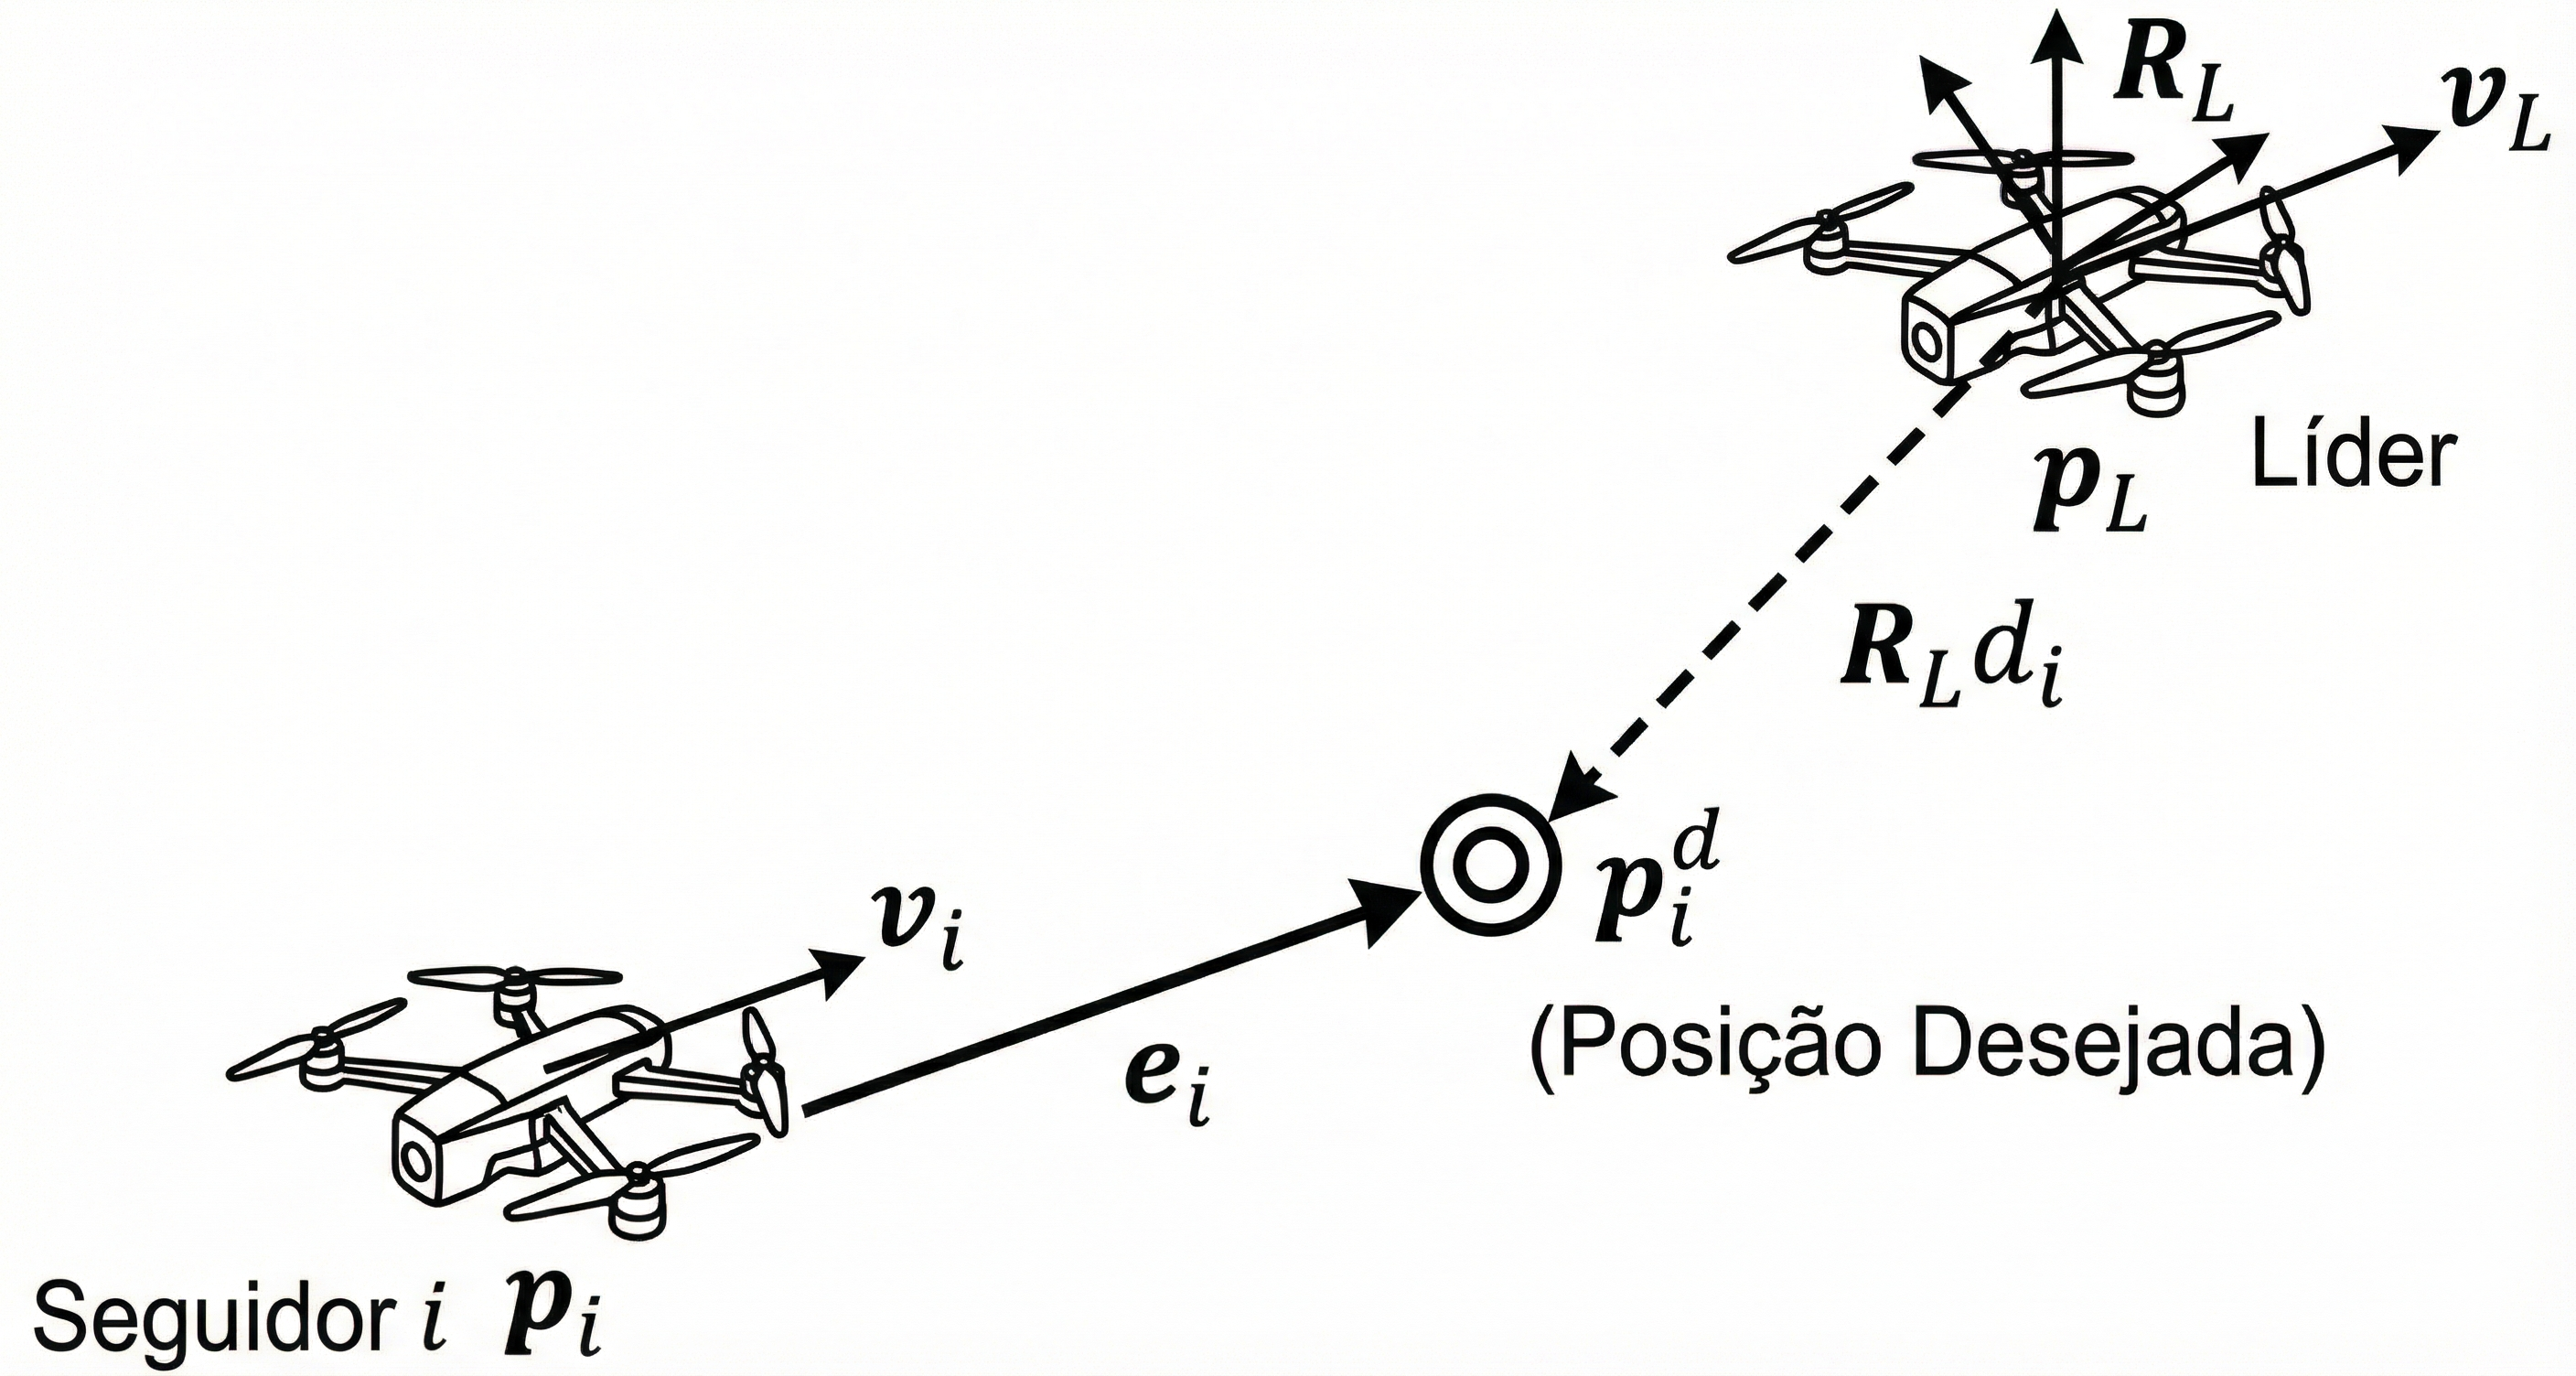
\includegraphics[width=0.7\linewidth]{images/Leader-Follower_pt.png}
    \caption{Representação do algoritmo Leader--Follower.}
    \label{fig:leader-follower}
\end{figure}

Apesar de sua simplicidade, o método é sensível à perda de comunicação ou falha do líder, o que pode comprometer a coesão do grupo. Abordagens mais recentes buscam mitigar essas limitações por meio de múltiplos líderes ou estratégias distribuídas de controle cooperativo.


\subsubsection{Virtual Structure}

Na estratégia \textit{Virtual Structure}, o grupo de VANTs é tratado como uma única estrutura rígida virtual, em que cada veículo ocupa uma posição fixa pré-definida dentro dessa estrutura \citep{bu2024advancement, askari2015virtualstructure}. O enxame, então, desloca-se como uma entidade unificada, preservando forma e orientação com elevada precisão.

Seja $p_v(t) \in \mathbb{R}^3$ a posição do centro da estrutura virtual e $R_v(t) \in SO(3)$ sua matriz de rotação, que define a orientação global da formação. Cada VANT $i$ possui um vetor $r_i^{VS}$ que especifica sua posição relativa fixa dentro da estrutura. Assim, a posição desejada do VANT $i$ é:

\begin{equation}
p_i^{d}(t) = p_v(t) + R_v(t)\, r_i^{VS}
\end{equation}

e a velocidade desejada segue da cinemática de corpo rígido, $v_i^{d}(t) = v_v(t) + \omega_v(t) \times \big( R_v(t)\, r_i^{VS} \big)$, onde $v_v(t)$ é a velocidade linear da estrutura virtual e $\times$ denota o produto vetorial entre a velocidade angular da estrutura virtual e a posição relativa do VANT expressa no referencial global. O controle de posição e velocidade de cada VANT é definido por uma lei de controle proporcional-derivativa (PD), dada por:

\begin{equation}
u_i = K_p (p_i^{d} - p_i) + K_d (v_i^{d} - v_i)
\end{equation}

onde $u_i$ representa o vetor de aceleração de controle do VANT $i$, e $K_p$, $K_d$ são matrizes de ganhos proporcionais e derivativos, respectivamente. Essa lei de controle assegura que cada VANT siga rigidamente o movimento da estrutura virtual, compensando desvios de posição e velocidade em relação à sua referência local dentro do corpo virtual. Assumindo uma dinâmica de segunda ordem $\ddot{p}_i = u_i$, o erro de posição $e_i = p_i^{d} - p_i$ evolui segundo $\ddot{e}_i + K_d \dot{e}_i + K_p e_i = 0$, o que caracteriza um sistema linear de segunda ordem estável se $K_p > 0$ e $K_d > 0$, garantindo convergência exponencial do erro para zero.

A principal vantagem dessa abordagem é a manutenção precisa da geometria da formação, mesmo em manobras complexas. Entretanto, ela requer sincronização e comunicação global entre os VANTs para garantir consistência no estado da estrutura virtual, o que pode limitar sua aplicação em cenários com comunicação intermitente ou ambientes altamente dinâmicos \citep{bu2024advancement, ouyang2023formation}.


\subsubsection{Behavior-Based}

A abordagem \textit{Behavior-Based} fundamenta-se em regras locais simples, inspiradas em sistemas biológicos como bandos de aves e cardumes de peixes \citep{balch2002behaviorbased}. Cada VANT ajusta seu movimento de forma autônoma com base em informações provenientes apenas de seus vizinhos mais próximos, seguindo comportamentos fundamentais de \textit{separação}, \textit{coesão}, \textit{alinhamento} e, em algumas aplicações, \textit{busca por objetivo} (\textit{goal seeking}) \citep{ouyang2023formation, reynolds1987flocks}.

A força de controle total aplicada ao agente $i$ é obtida pela soma ponderada dos vetores de cada comportamento:

\begin{equation}
u_i = w_s f_{sep,i} + w_c f_{coh,i} + w_a f_{ali,i} + w_g f_{goal,i}
\end{equation}

onde $w_s$, $w_c$, $w_a$ e $w_g$ são os pesos que determinam a influência relativa do comportamento de Separação, Coesão, Alinhamento e Busca por objetivo, respectivamente. Os vetores de controle são definidos como:

\begin{equation}
\begin{aligned}
f_{sep,i} &= \sum_{j \in N_i} \frac{p_i - p_j}{\|p_i - p_j\|^2} && \text{(Separação)} \\[6pt]
f_{coh,i} &= \frac{1}{|N_i|}\sum_{j \in N_i}(p_j - p_i) && \text{(Coesão)} \\[6pt]
f_{ali,i} &= \frac{1}{|N_i|}\sum_{j \in N_i}(v_j - v_i) && \text{(Alinhamento)} \\[6pt]
f_{goal,i} &= p_{goal} - p_i && \text{(Busca por objetivo)}
\end{aligned}
\end{equation}

O comportamento de \textit{separação} evita colisões e mantém espaçamento mínimo seguro entre os VANTs; o de \textit{coesão} busca preservar a unidade do grupo; o de \textit{alinhamento} sincroniza a direção de voo com a média dos vizinhos; e o de \textit{busca por objetivo} conduz o enxame a um alvo ou trajetória desejada. A dinâmica de cada agente é descrita por $\dot{p}_i = v_i$ e $\dot{v}_i = u_i$, onde $p_i$ e $v_i$ são, respectivamente, a posição linear e a velocidade linear do VANT $i$; assim, o vetor $u_i$ representa a aceleração desejada calculada a partir da combinação dos comportamentos locais.

Essa formulação resulta em um sistema de controle totalmente distribuído, no qual o comportamento coletivo emerge das interações locais entre agentes. Tal característica garante escalabilidade e robustez a falhas de comunicação, mas dificulta a manutenção de formações geométricas rígidas e a obtenção de estabilidade formal em cenários complexos \citep{bu2024advancement, ouyang2023formation}.

\subsubsection{Consensus-Based}

Os métodos \textit{Consensus-Based} têm como objetivo permitir que todos os VANTs atinjam um acordo (\textit{consenso}) sobre variáveis de estado, como posição, velocidade ou orientação, utilizando apenas informações locais de vizinhança \citep{bu2024advancement, ouyang2023formation, olfati2007consensus, ren2008distributed}. 

A topologia de comunicação entre os VANTs é representada por um grafo direcionado \(\mathcal{G} = (\mathcal{V}, \mathcal{E})\), onde \(\mathcal{V} = \{1, 2, \dots, N\}\) é o conjunto de agentes e \(\mathcal{E} \subseteq \mathcal{V} \times \mathcal{V}\) define as conexões entre eles. Na matriz de adjacência \(A = [a_{ij}]\in\mathbb{R}^{N\times N}\), tem-se \(a_{ij} > 0\) se existe a aresta \((j,i)\in\mathcal{E}\) e \(a_{ij} = 0\) caso contrário; ou seja, a entrada \(a_{ij}\) representa o peso com que a informação do agente \(j\) é considerada pelo agente \(i\). Definindo o grau (in-degree) de cada agente como \(d_i = \sum_{j=1}^{N} a_{ij}\) e a matriz diagonal dos graus \(D=\mathrm{diag}(d_1,\dots,d_N)\), a matriz Laplaciana é dada por \(L = D - A\). Denota-se ainda por \(\mathcal{N}_i = \{\, j \in \mathcal{V} \mid a_{ij} > 0 \,\}\) o conjunto de vizinhos que enviam informação ao agente \(i\) (às vezes chamado de \emph{in-neighborhood} de \(i\)).

\paragraph{Modelagem para agentes de primeira ordem.}
Considerando que cada agente \(i\) possui um estado \(x_i(t)\) e que sua dinâmica é dada por \(\dot{x}_i = u_i\), o controle de consenso é expresso por:

\begin{equation}
u_i = -\sum_{j \in \mathcal{N}_i} a_{ij} (x_i - x_j),
\end{equation}

o que resulta, na forma vetorial compacta, em \(\dot{x} = -Lx\), onde \(x = [x_1, x_2, \dots, x_N]^T\). Quando o grafo é fortemente conexo, o sistema garante a convergência para o consenso global, isto é, \(\lim_{t \to \infty} (x_i(t) - x_j(t)) = 0\) para todo \(i,j\).

\paragraph{Modelagem para agentes de segunda ordem.}
Em sistemas mais realistas, como enxames de VANTs, é necessário considerar tanto a posição \(p_i\) quanto a velocidade \(v_i\) de cada agente, com dinâmica de segunda ordem \(\dot{p}_i = v_i\) e \(\dot{v}_i = u_i\). O controle de consenso estendido para esse caso pode ser expresso como:

\begin{equation}
u_i = -k_p \sum_{j \in \mathcal{N}_i} a_{ij}(p_i - p_j) - k_v \sum_{j \in \mathcal{N}_i} a_{ij}(v_i - v_j),
\end{equation}

em que \(k_p\) e \(k_v\) são ganhos de acoplamento que determinam a velocidade de convergência da formação. Sob condições de conectividade adequadas do grafo, as diferenças \(p_i - p_j\) e \(v_i - v_j\) tendem a zero para todo \(i,j\), ou seja, todos os VANTs convergem para a mesma trajetória e velocidade, atingindo consenso tanto em posição quanto em movimento.

Essa abordagem apresenta uma base teórica sólida e comprovada estabilidade quando o grafo de comunicação é conexo. Sua simplicidade, robustez e escalabilidade tornam o método \textit{Consensus-Based} amplamente utilizado em aplicações de coordenação distribuída, controle de formação e sincronização em redes multiagente \citep{olfati2007consensus, ren2008distributed}.


\subsubsection{Artificial Potential Fields}

O método dos \textit{Artificial Potential Fields} (APF) propõe o uso de campos de potencial artificiais para gerar forças virtuais de atração e repulsão que guiam o movimento dos agentes de forma contínua e descentralizada \citep{khatib1986real, bu2024advancement, ouyang2023formation}. Nesse contexto, o ambiente é modelado como um campo energético, em que o objetivo atua como uma fonte atrativa e os obstáculos ou demais VANTs funcionam como fontes repulsivas.

O potencial total associado ao agente $i$ é definido por $U_i(p_i) = U_{att}(p_i) + U_{rep}(p_i)$, em que o termo atrativo $U_{att}(p_i)$ direciona o VANT para o alvo e o termo repulsivo $U_{rep}(p_i)$ evita colisões com obstáculos e vizinhos próximos. O potencial atrativo é geralmente modelado de forma quadrática, $U_{att}(p_i) = \frac{1}{2} k_{att} \|p_i - p_{goal}\|^2$, onde $k_{att} > 0$ representa o ganho de atração e $p_{goal}$ a posição desejada. Já o potencial repulsivo atua apenas dentro de uma distância de influência $d_0$, sendo dado por:

\begin{equation}
U_{rep}(p_i) =
\frac{1}{2} k_{rep} 
\sum_{j \in N_i}
\left(
\frac{1}{\|p_i - p_j\|} - \frac{1}{d_0}
\right)^2
\mathbb{I}_{\|p_i - p_j\| < d_0}
\end{equation}

onde $k_{rep} > 0$ é o ganho de repulsão, $N_i$ representa o conjunto de vizinhos do agente $i$, e $\mathbb{I}$ é a função indicadora, que vale 1 quando a condição é verdadeira e 0 caso contrário. A força resultante que governa o movimento do agente é obtida pelo gradiente negativo do potencial total, $f_i = -\nabla U_i = f_{att,i} + f_{rep,i}$, com:

\begin{equation}
\begin{split}
f_{att,i} &= -k_{att}(p_i - p_{goal}), \\
f_{rep,i} &= 
\sum_{j \in N_i} k_{rep}
\left(\frac{1}{\|p_i - p_j\|} - \frac{1}{d_0}\right)
\\
&\quad\times
\frac{1}{\|p_i - p_j\|^3}(p_i - p_j)
\mathbb{I}_{\|p_i - p_j\| < d_0}
\end{split}
\end{equation}

Com a dinâmica de movimento $\dot{p}_i = v_i$ e $\dot{v}_i = f_i$, cada VANT ajusta sua aceleração de acordo com o gradiente do campo de potencial. Essa formulação permite que as formações se reorganizem em tempo real e evitem colisões, mesmo em ambientes dinâmicos. No entanto, o método pode apresentar limitações devido à presença de mínimos locais — situações em que o potencial total apresenta pontos de equilíbrio indesejados que impedem a convergência ao objetivo \citep{khatib1986real, bu2024advancement, ouyang2023formation}. Uma representação da abordagem APF é mostrada na Figura~\ref{fig:APF}.

\begin{figure}[ht]
    \centering
    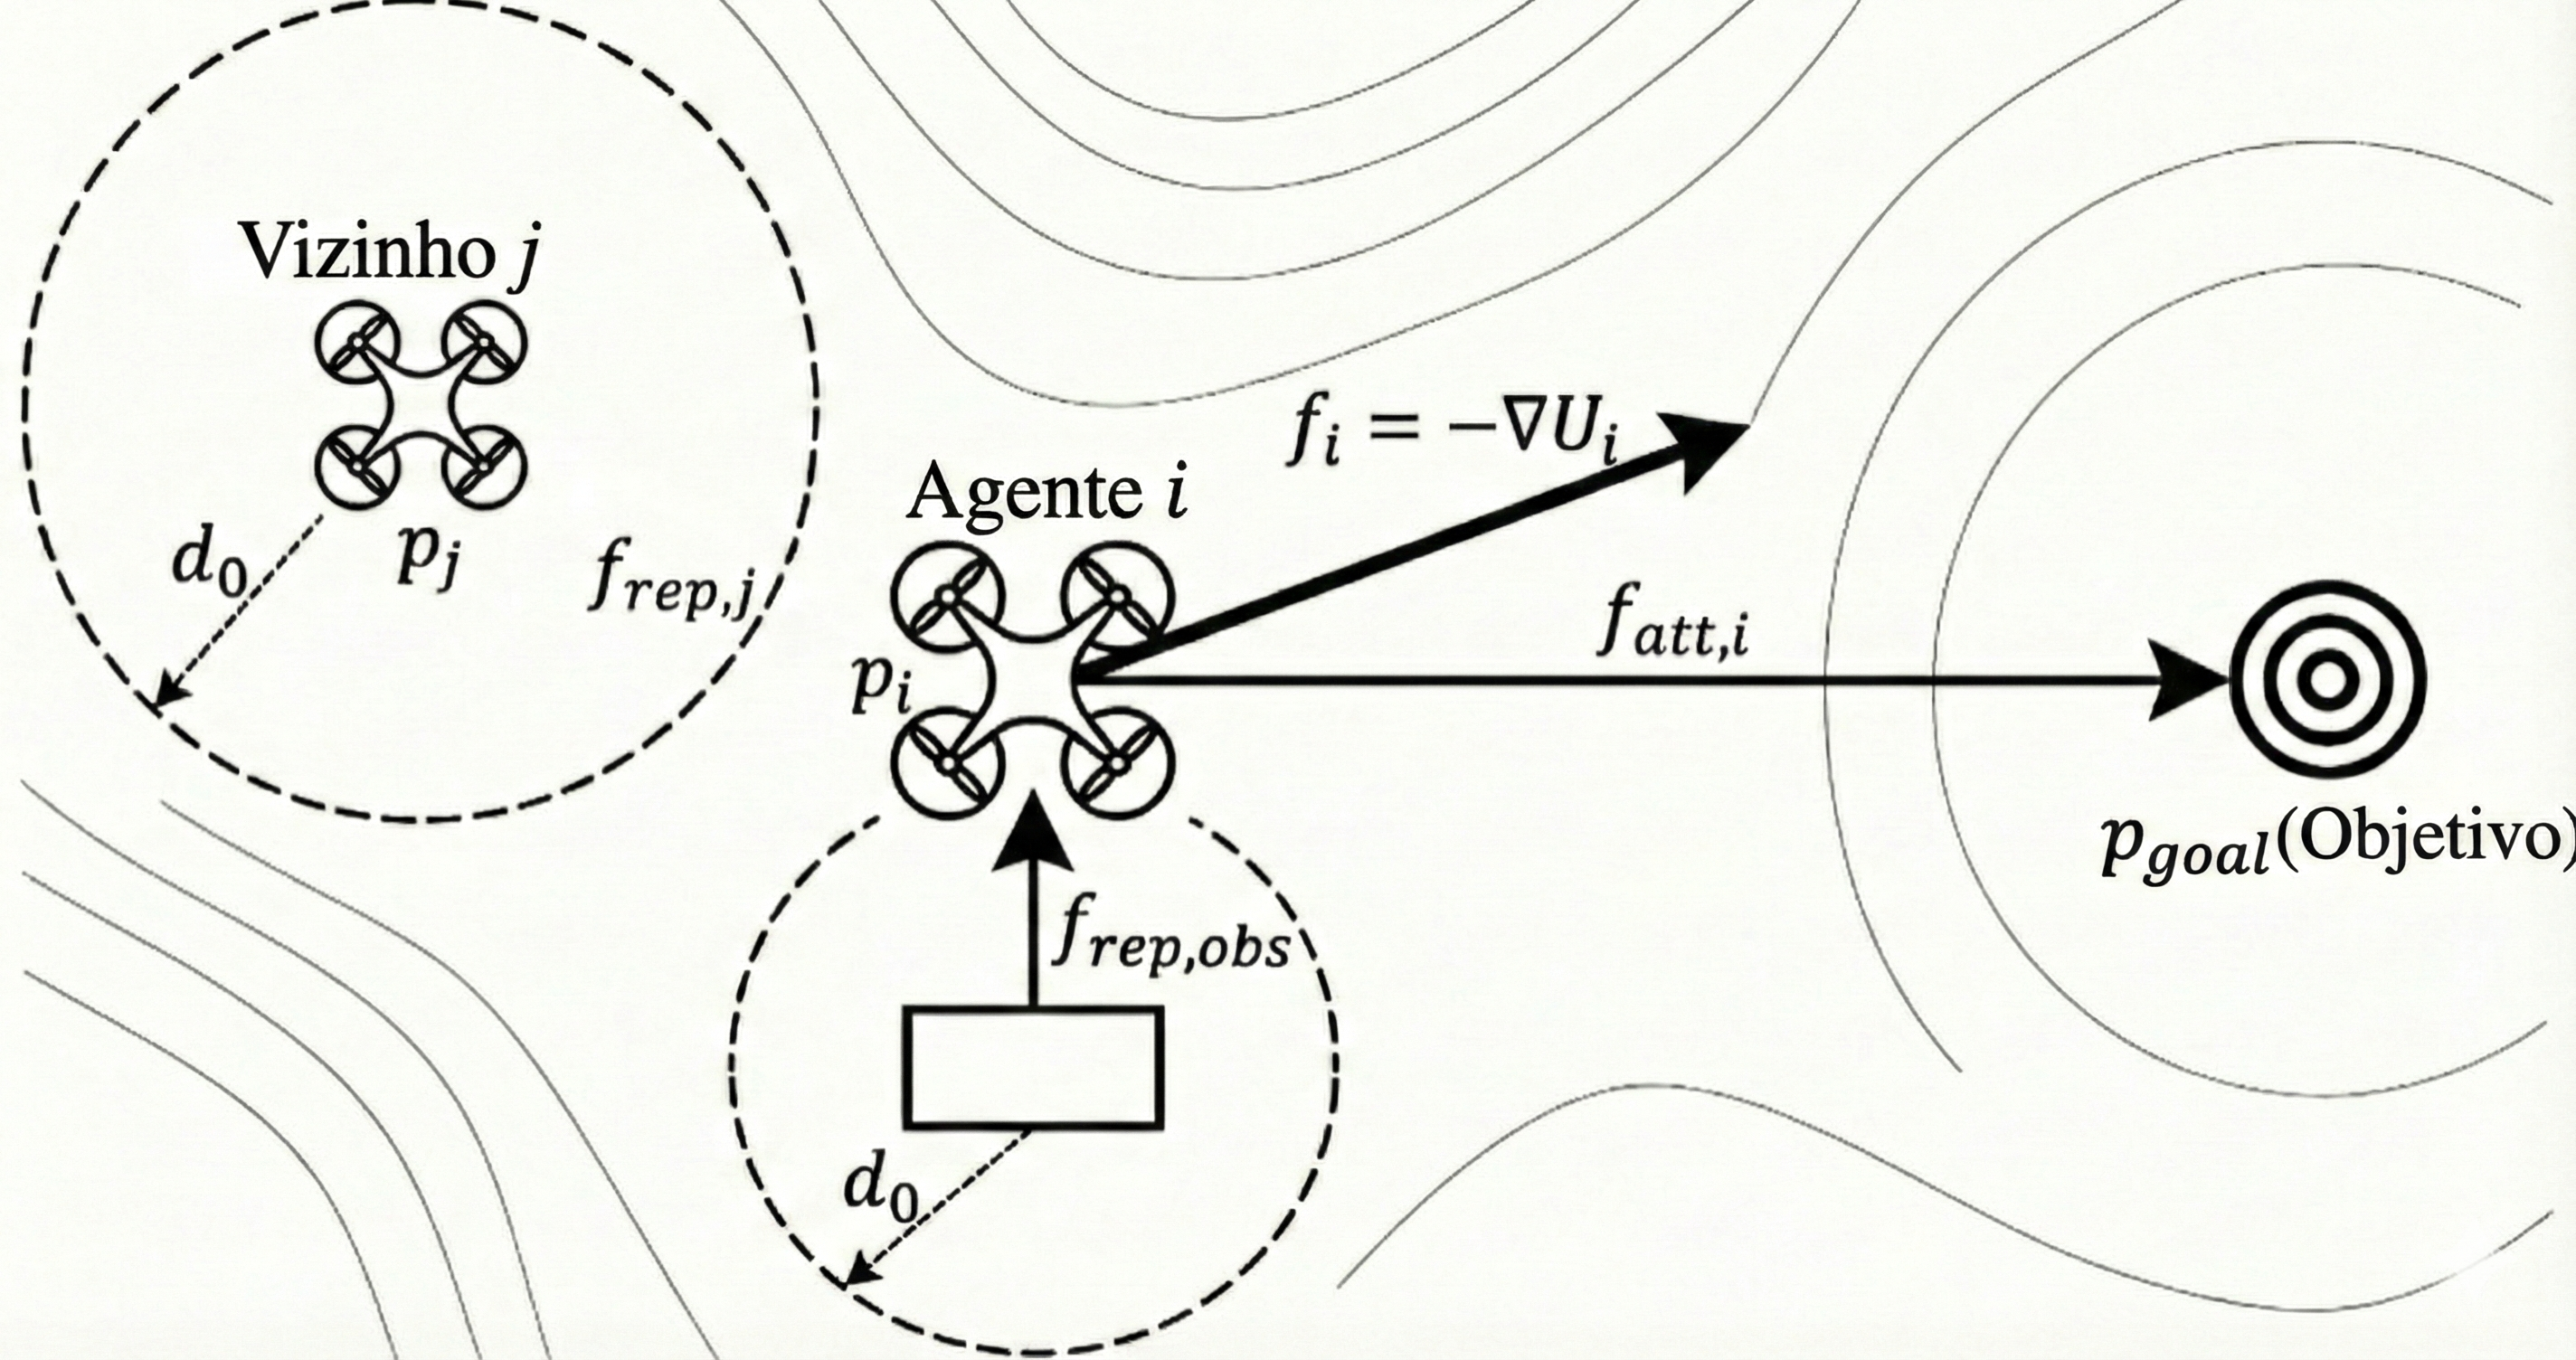
\includegraphics[width=1.0\linewidth]{images/APF_pt.png}
    \caption{Representação do algoritmo APF.}
    \label{fig:APF}
\end{figure}

\subsubsection*{Comparação Geral}

Cada uma dessas abordagens apresenta vantagens específicas. Os métodos \textit{Leader–Follower} e \textit{Virtual Structure} são indicados para formações bem definidas e controladas centralmente, enquanto as estratégias \textit{Behavior-Based}, \textit{Consensus-Based} e \textit{Artificial Potential Fields} são mais adequadas para ambientes dinâmicos e distribuídos. Em sistemas reais, é comum a combinação híbrida entre métodos, buscando equilibrar estabilidade, escalabilidade e adaptabilidade \citep{bu2024advancement, ouyang2023formation}.

\subsection{Comunicação e Simulação de Enxames de VANTs}

A comunicação é um elemento essencial para a coordenação de enxames de VANTs, que frequentemente operam em redes ad hoc conhecidas como FANETs (\textit{Flying Ad Hoc Networks}) \citep{khan2017fanet, hong2020swarm}. Essas redes caracterizam-se por alta mobilidade, auto-organização e ausência de controle centralizado; a dinâmica tridimensional dos VANTs, associada a velocidades de deslocamento de 30 a 460 km/h, resulta em rápidas variações na topologia da rede e exige protocolos de comunicação resilientes \citep{khan2017fanet}. Nesse contexto, o protocolo \textit{MAVLink}, amplamente utilizado em sistemas \textit{open-source} como PX4 e ArduPilot, provê uma camada leve de comunicação baseada em mensagens entre o sistema de controle de voo e a estação terrestre \citep{Young-Min2018}, enquanto o \textit{ROS} e o \textit{ROS2} --- este baseado em DDS (\textit{Data Distribution Service}) e em arquitetura totalmente distribuída --- fornecem uma infraestrutura modular que viabiliza a integração de múltiplos agentes, sensores e atuadores \citep{khaliq2021, ziming2023}. Ainda assim, a comunicação entre VANTs permanece sujeita a latência, perda de pacotes e ataques de rede: estudos experimentais mostraram que ataques de saturação podem aumentar a variância do tempo de recepção de dados em mais de 30 vezes, afetando diretamente o desempenho dos controladores de formação \citep{Young-Min2018}.

As plataformas de simulação são ferramentas essenciais para desenvolver e validar essas estratégias, pois permitem testar algoritmos de formação, sincronização e evasão de obstáculos em ambientes virtuais, reduzindo custos e riscos associados a testes reais \citep{khaliq2021, ziming2023}. Simuladores como \textit{Gazebo}, \textit{Webots}, \textit{CoppeliaSim} e o \textit{SITL PX4} fornecem ambientes tridimensionais realistas para a modelagem de cenários de voo e formação \citep{ziming2023}; o \textit{Gazebo}, em particular, integra-se ao \textit{ROS}/ROS~2 para simulações \textit{Software-In-The-Loop} (SIL) e \textit{Hardware-In-The-Loop} (HIL) \citep{khaliq2021}. Nessas simulações, o MAVLink atua como protocolo de mensageria entre os nós simulados e cada VANT emulado executa seu próprio nó ROS/ROS~2 \citep{khaliq2021, ROS2Design2022}, enquanto a modelagem de sensores e ambientes permite incluir ruído, atraso de comunicação e falhas de hardware simuladas \citep{ziming2023, PX4SITL2024}. Essa integração entre simulação física, autopiloto em modo SITL e rede distribuída fundamenta a arquitetura de simulação adotada neste trabalho, descrita na Seção~\ref{sec:metodologia}.

\subsection{Síntese e Direcionamento do Trabalho}

A fundamentação teórica apresentada integrou os principais conceitos relacionados à comunicação, coordenação, simulação e controle de formação em enxames de VANTs. Os protocolos de comunicação, como o \textit{MAVLink} e o \textit{ROS/ROS2}, fornecem a base para a interoperabilidade e sincronização entre múltiplos agentes; sobre essa infraestrutura, os algoritmos de formação --- como os baseados em consenso, comportamento e estruturas virtuais --- determinam a dinâmica coletiva dos VANTs, regulando como o grupo se organiza, mantém coesão e responde a perturbações externas; e as plataformas de simulação, como o \textit{Gazebo} e o \textit{SITL PX4}, tornam possível testar e validar essas estratégias em cenários controlados, antes de sua aplicação em experimentos reais \citep{ouyang2023formation, bu2024advancement, khaliq2021}. Com base nessa revisão, a Seção~\ref{sec:metodologia} descreve como esses algoritmos, e a hibridização entre eles, foram comparados em diferentes cenários de simulação.

